Fairness entails more than the question whether are lottery numbers from the expected distribution. For instance, the Kolmogorov-Smirnov
test used in the first part of this paper does not concern itself with the order the numbers are drawn. However if we saw a lottery whose
numbers were always drawn in a descending sequence, for example, we would become suspicious.

Thus a more comprehensive test is clearly required to establish a more detailed answer to our question. We approach this problem by reformulating
lottery as a process producing a stream of (supposedly) random numbers, which themselves are simply bit sequences. Under this formulation,
we can deploy standard statistical tests developed for testing random number generators: we have a file of one and zero bits and wish to investigate
if its bits are correlated, repeating with a period or other quantities undesirable for randomness.

A number of these test suites has been developed over time. Donald Knuth presented an initial set of empirical tests in the second volume of his computer science bible
The Art of Computer Programming in 1969. Many general cryptography textbooks such as \href{http://www.cacr.math.uwaterloo.ca/hac/}{Handbook of Applied Cryptography} 
or \href{http://www.wisdom.weizmann.ac.il/~oded/foc-vol1.html}{Foundations of Cryptography} contain multiple tests of their own. The american National Institute 
of Standards \& Technology has published a \href{https://nvlpubs.nist.gov/nistpubs/legacy/sp/nistspecialpublication800-22r1a.pdf}{guideline} discussing this matter too.

We decided to use the Diehard battery of tests, which was developed by the american statistician George Marsaglia in the nineties. While this package used
to be quite popular in its day, it has been superceded today by other suites, including its derivatives such as Dieharder or TestU01. In comparison with the alternatives,
the Diehard tests \href{https://crypto.stackexchange.com/questions/90076/how-to-compute-the-dataset-size-required-by-dieharder-tests}{consume a lot less data}, making
its use feasible to limited data cases such as our project.

Nonetheless even less data greedy test still requires quite a lot of data. We are thus limited in which tests we can run, see~\ref{fig:dataset} for our dataset size.

\begin{figure}
    \centering
    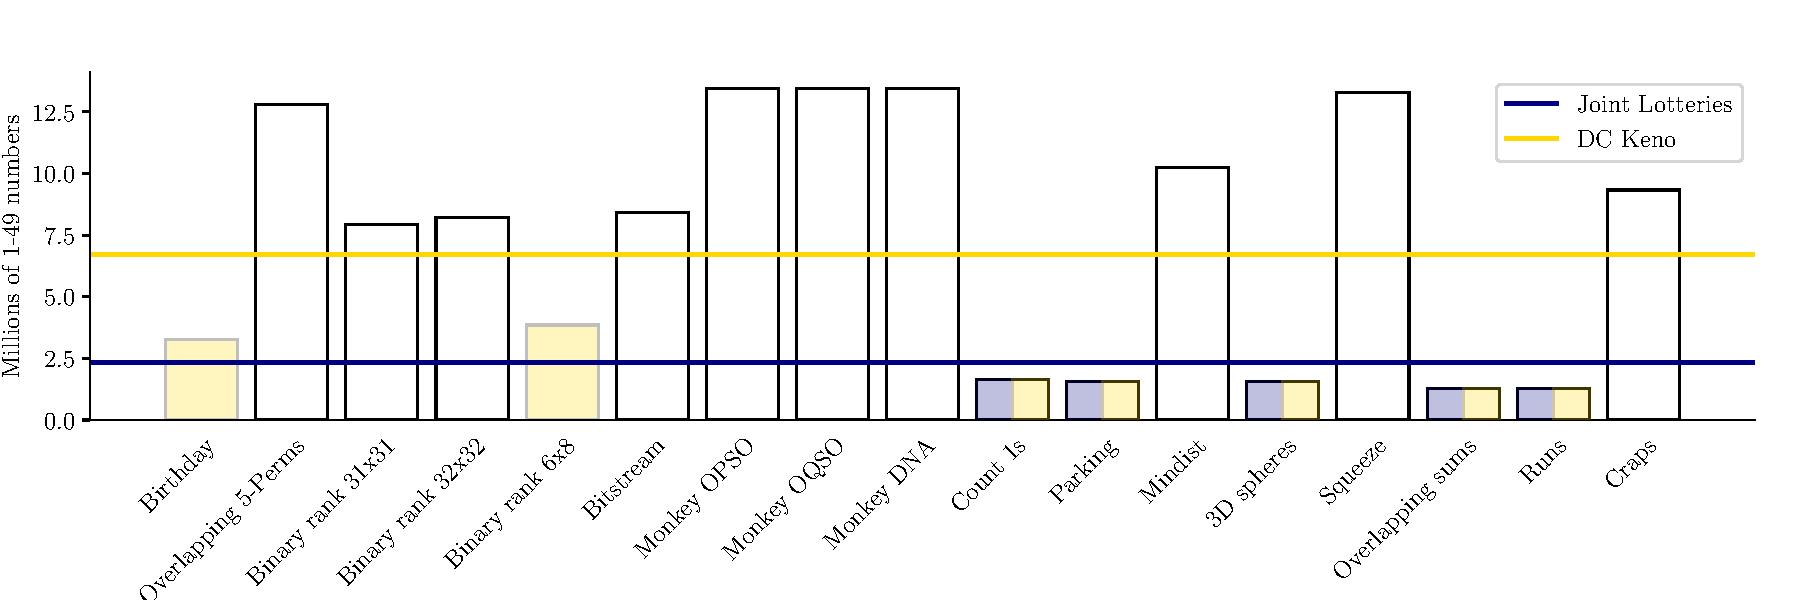
\includegraphics[width=\textwidth]{diehard_requirements.pdf}
    \caption{Amount of data required to run tests at default settings.}
    \label{fig:requirements}
\end{figure}

\subsection{Data augmentation}

Diehard battery expects a random stream of zero and one bits as input. To satisfy this, we transform our lottery numbers distributed in 1-n range by first
subtracting 1 and taking 5 lowest bits from every number for $n \in \langle 32, 64)$ or 6 for $n \in \langle 64, 128)$.

This transformation doesn't however solve all problems. The winning numbers are sometimes provided in sorted, ascending order in a single draw. We discuss
this in further sections. Furthermore, the numbers are drawn without replacement. We argue that this is an acceptable deviation. \todo{A bit of combinatorics,
combinations with replacement as approximation for combinations without replacement}.

\subsection{Results}

\begin{figure}
    \centering
    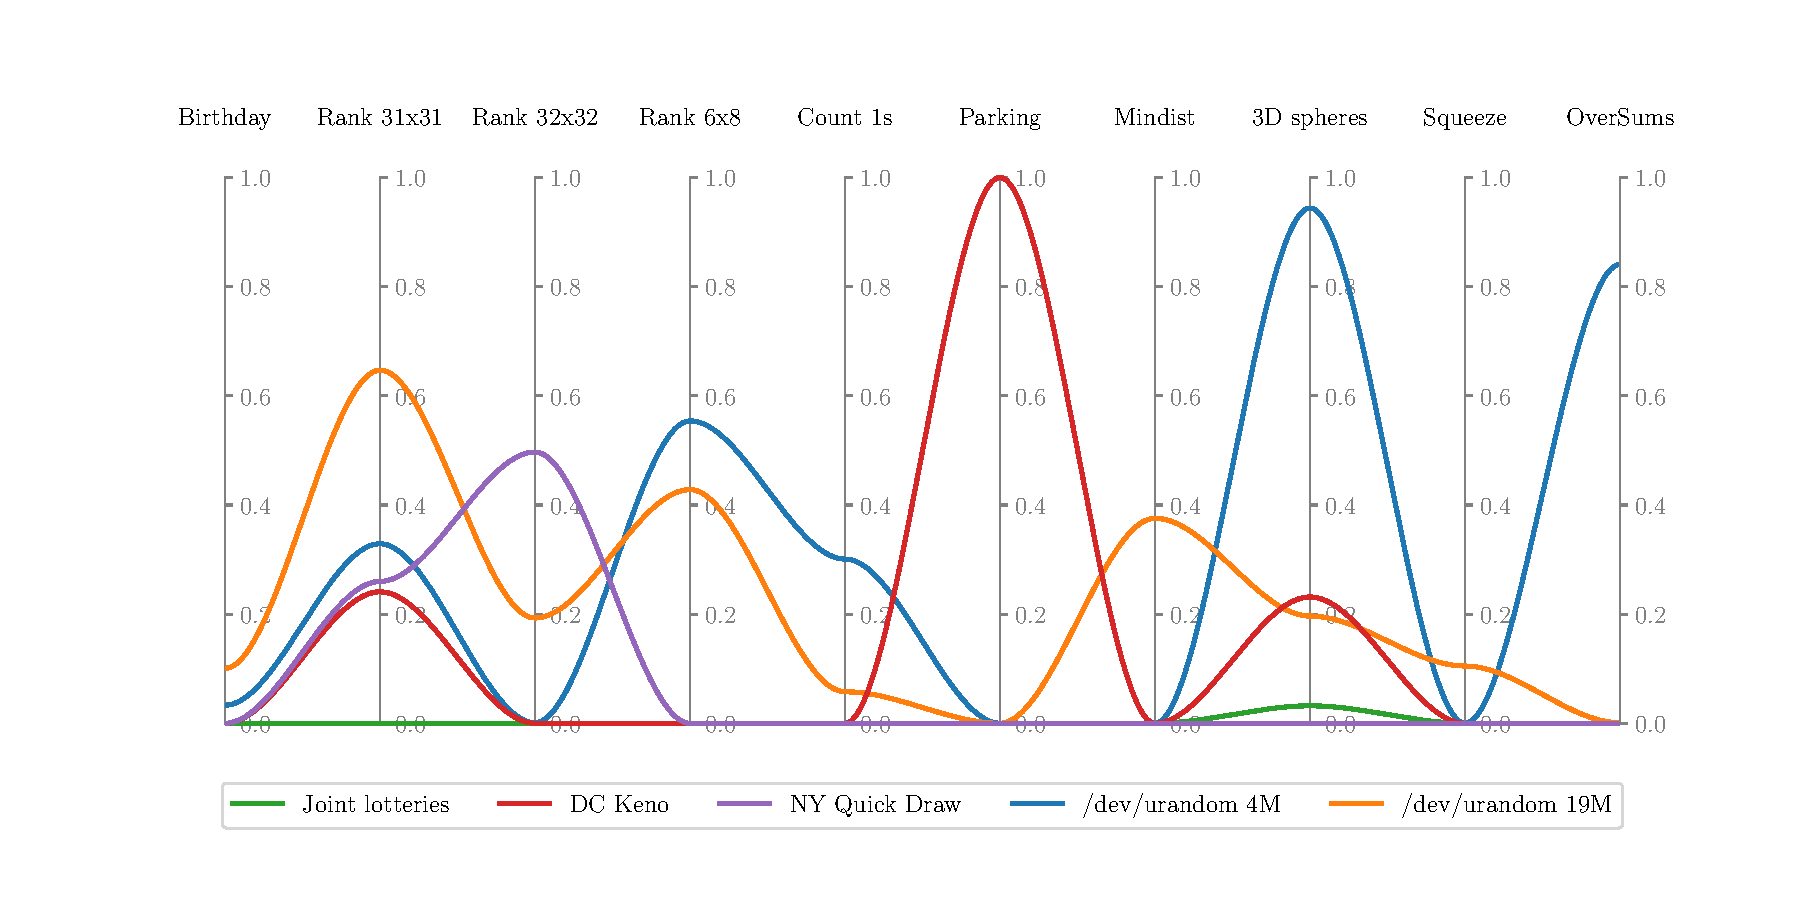
\includegraphics[width=\textwidth]{performance.pdf}
    \caption{Score at various Diehard tests.}
    \label{fig:performance}
\end{figure}

\begin{figure}
    \centering
    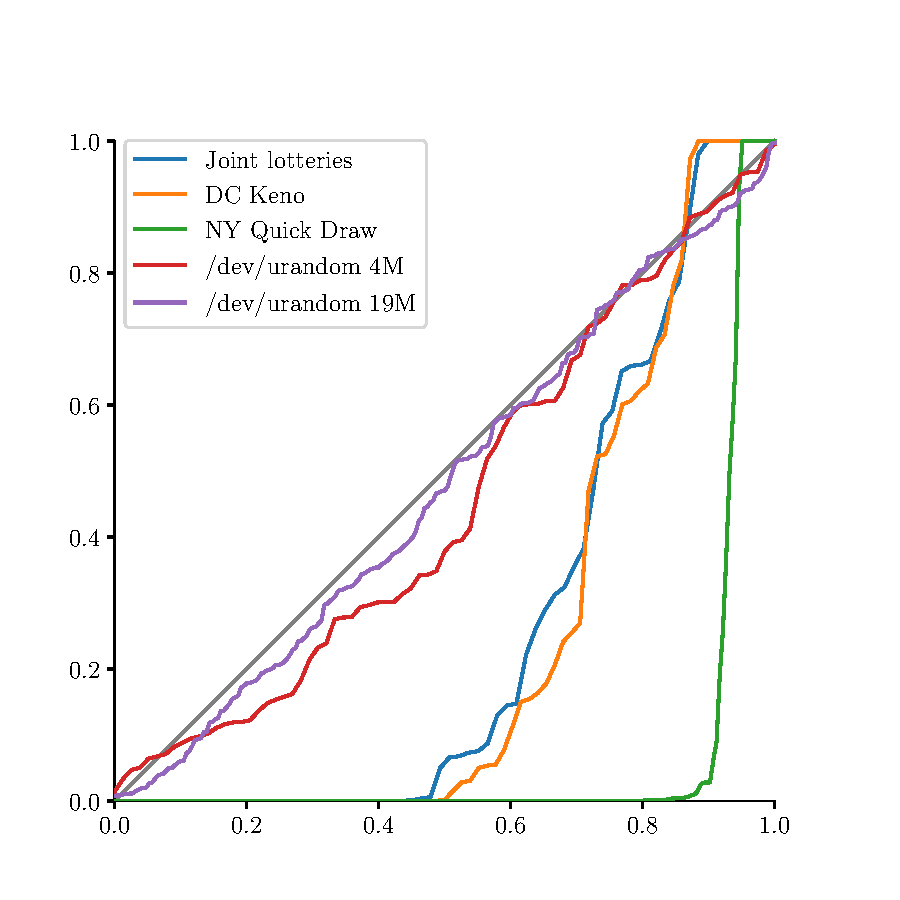
\includegraphics[width=\textwidth]{pvalue_distribution.pdf}
    \caption{Randomness quality as measured by Diehard. Gray line is perfect randomness.}
    \label{fig:pvalue_distribution}
\end{figure}

\begin{enumerate}
    \item About Diehard.
    \item The following part is divided into several section. In section 1, we discuss data gathering, processing and general creation of input files for Diehard. Special
    attention is given to the problem of attaining input file of sufficient size and the asymetric requirements of individual Diehard tests.
    \item Part 2 highlights result on Diehard suite, interprets them and compares them against commonly used PRNGs.
    \item Section 3 clarifies the shortcomings of above approach.
\end{enumerate}
